\documentclass{article}
\usepackage{dcolumn}
\usepackage{booktabs}
\usepackage{tikz}
\usetikzlibrary{positioning,shapes,arrows}

\newcolumntype{M}[1]{D{.}{.}{1.#1}}

\begin{document}
	
	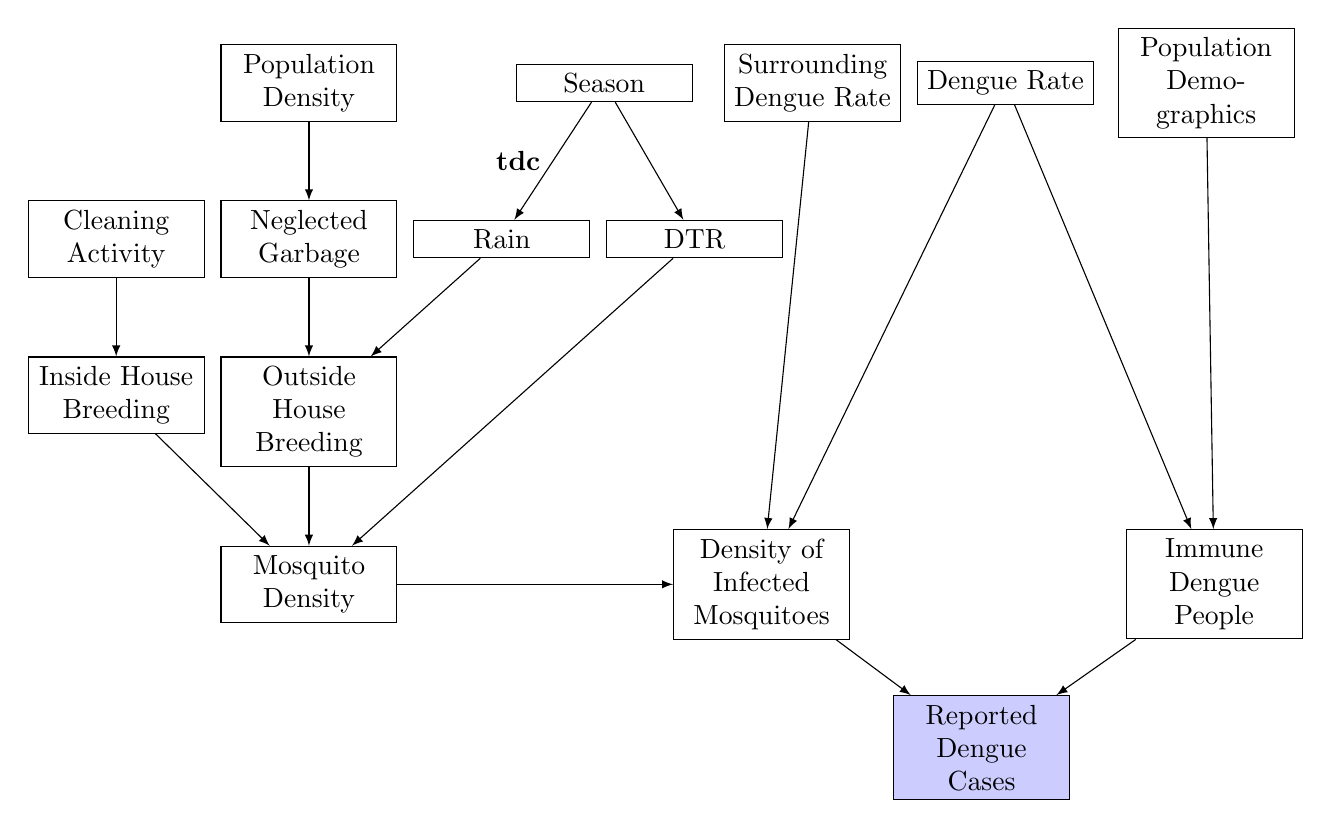
\begin{tikzpicture}[
	node distance=1cm and 0cm,
	mynode/.style={draw,  rectangle, text width=2cm,align=center}
	]
		
	\node[mynode] (pd) {Population Density};	
    \node[mynode,below =of pd]  (grb){Neglected Garbage};
    \node[mynode,left = 0.2 cm of grb]  (ca){Cleaning Activity};
    \node[mynode,below =of grb]  (ob){Outside House Breeding};
    \node[mynode,below =of ca]  (ib){Inside House Breeding};
    \node[mynode,below  = of ob]  (md){Mosquito Density};
    
    \node[mynode, right = 1.5 cm of pd]  (season){Season};
    \node[mynode, below left = of season, right = 0.2 cm of grb]  (rain){Rain};
    \node[mynode, below right = of season, right = 0.2 cm of rain]  (DTR){DTR};
    
    
    
    \node[mynode, right = 0.4 cm of season]  (mndr){Surrounding Dengue Rate};
    \node[mynode, right = 0.2 cm of mndr]  (dr){Dengue Rate};
    \node[mynode, right = 0.3 cm of dr]  (pdr){Population Demographics};
    
    \node[mynode,right = 3.5 cm of md]  (dim){Density of Infected Mosquitoes};
    \node[mynode,right = 3.5 cm of dim]  (idp){Immune Dengue People};
    
    \node[mynode,below left = 1cm of idp, fill=blue!20]  (dh){Reported Dengue Cases};
    
    

	\path (season) edge[-latex, ] node[left=1pt] {\textbf{tdc}}   (rain)
	(season) edge[-latex] (DTR)  
	(rain) edge[-latex] (ob)
	(DTR) edge[-latex] (md)
	(dr) edge[-latex] (idp)
	(pdr) edge[-latex] (idp)
	(dr) edge[-latex] (dim)
	(mndr) edge[-latex] (dim)
	
	
	(pd) edge[-latex] (grb)
	(grb) edge[-latex] (ob)
	(ob) edge[-latex] (md) 
	(ib) edge[-latex] (md) 
	(md) edge[-latex] (dim)
	(dim) edge[-latex] (dh)
	(idp) edge[-latex] (dh)
	(ca) edge[-latex] (ib);
		
	\end{tikzpicture}
	
\end{document}
